\documentclass[11pt,a4paper]{article}

\usepackage[utf8]{inputenc}
\usepackage[T1]{fontenc}
\usepackage{mathpazo}
\usepackage[scaled=0.92]{helvet}
\usepackage[margin=1in]{geometry}
\usepackage{graphicx}
\usepackage{amsmath,amssymb,amsfonts}
\usepackage{booktabs}
\usepackage{tabularx}
\usepackage{setspace}
\usepackage{titlesec}
\usepackage{fancyhdr}
\usepackage{float}
\usepackage{caption}
\usepackage{microtype}

\usepackage{tikz}
\usetikzlibrary{shapes.geometric, arrows.meta, positioning, calc, matrix}

\usepackage{listings}
\usepackage{xcolor}
\usepackage[hidelinks]{hyperref}

% --- SETUP (Sesuai dengan Paper Anda) ---
\setstretch{1.15}
\setlength{\parindent}{0pt}
\setlength{\parskip}{0.8em}
\sloppy

\titleformat{\section}{\normalfont\large\bfseries\sffamily}{\thesection}{1em}{}
\titleformat{\subsection}{\normalfont\normalsize\bfseries\sffamily}{\thesubsection}{1em}{}

\pagestyle{fancy}
\fancyhf{}
\fancyhead[L]{\small\sffamily Fondasi Basis Data: Tipe Data SQL}
\fancyhead[R]{\small\sffamily\thepage}
\renewcommand{\headrulewidth}{0.4pt}

\captionsetup{font=small,labelfont=bf,labelsep=period}

\renewenvironment{abstract}
{\small
	\begin{center}\textbf{\sffamily Abstrak}\end{center}
	\begin{quote}}
	{\end{quote}}

\title{\vspace{-1.5cm}\textbf{\sffamily\LARGE Fondasi Basis Data: Memahami Tipe Data SQL secara Mendalam}}
\author{
	\textbf{Muhammad Riduwan Khafidi} \\
	\small Program Studi Teknik Rekayasa Perangkat Lunak \\
	\small Politeknik Negeri Batam \\
	\small \texttt{4342611034@students.polibatam.ac.id}
}
\date{\small\today}

\begin{document}

\maketitle
\thispagestyle{empty}

\begin{abstract}
	Tipe data (\textit{data type}) bagaikan "jenis wadah" yang menentukan bagaimana sebuah nilai disimpan, dihitung, dan diinterpretasikan oleh mesin basis data. Salah memilih tipe data ibarat menyimpan air di dalam keranjang rotan: data bisa hilang (presisi berkurang) atau memboroskan ruang. Makalah ini membahas tipe data SQL bukan sekadar sebagai daftar hafalan, melainkan melalui pendekatan asosiatif dan visual. Pembaca akan diajak memahami analogi alokasi memori pada \texttt{CHAR} vs \texttt{VARCHAR}, bahaya tersembunyi di balik \texttt{FLOAT}, serta panduan praktis dalam memilih tipe data yang tepat untuk berbagai studi kasus nyata.
\end{abstract}

\section{Pendahuluan: Analogi Dasar Tipe Data}

Bayangkan Anda sedang mengemas barang untuk pindahan. Anda memiliki baju, dokumen penting, dan barang pecah belah. Anda tidak mungkin memasukkan baju ke dalam kotak kaca tipis, dan Anda tidak perlu memasukkan batu bata ke dalam kotak berlapis busa.

Dalam basis data, **Tipe Data adalah kotak kemasannya**. Memilih tipe data yang tepat menjamin tiga hal:
\begin{enumerate}
	\item \textbf{Integritas Data}: Memastikan hanya nilai yang valid yang bisa masuk (misal: kolom usia tidak bisa diisi teks "Dua Puluh").
	\item \textbf{Efisiensi Memori}: Menghemat ruang penyimpanan \textit{disk} dan memori RAM.
	\item \textbf{Kecepatan Akses}: Operasi aritmatika pada angka jauh lebih cepat daripada operasi pada teks.
\end{enumerate}

\section{Kategori Utama Tipe Data}

Secara garis besar, SQL membagi tipe datanya menjadi beberapa keluarga besar. Memahami keluarga ini memudahkan kita mengingat jenis-jenisnya.

\begin{figure}[H]
	\centering
	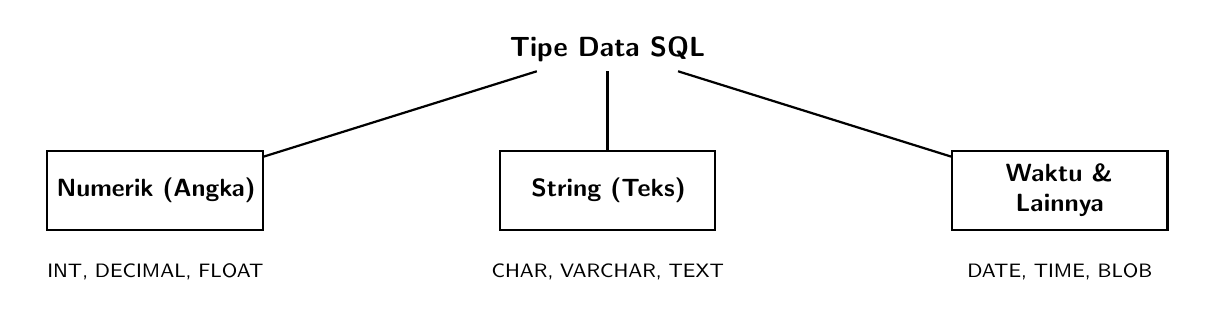
\begin{tikzpicture}[
			node distance=0.4cm and 1cm,
			cat/.style={rectangle, draw=black, thick, fill=white, text width=2.5cm, align=center, minimum height=1cm, font=\sffamily\small\bfseries},
			line/.style={draw, thick, -}
		]
		% Root
		\node[font=\sffamily\bfseries] (root) {Tipe Data SQL};

		% Level 1
		\node[cat, below left=1cm and 3cm of root] (num) {Numerik (Angka)};
		\node[cat, below=1cm of root] (str) {String (Teks)};
		\node[cat, below right=1cm and 3cm of root] (date) {Waktu \& Lainnya};

		% Level 2 (Koneksi)
		\draw[line] (root) -- (num);
		\draw[line] (root) -- (str);
		\draw[line] (root) -- (date);

		% Keterangan di bawah (bukan anak panah, tapi list)
		\node[below=0.3cm of num, font=\scriptsize\sffamily, text width=3cm, align=center] {INT, DECIMAL, FLOAT};
		\node[below=0.3cm of str, font=\scriptsize\sffamily, text width=3cm, align=center] {CHAR, VARCHAR, TEXT};
		\node[below=0.3cm of date, font=\scriptsize\sffamily, text width=3cm, align=center] {DATE, TIME, BLOB};
	\end{tikzpicture}
	\caption{Peta Keluarga Tipe Data SQL.}
\end{figure}

\section{Tipe Data Numerik: Presisi adalah Kunci}

Angka terbagi menjadi dua dunia: angka yang dapat dihitung secara pasti (\textit{exact}) dan angka yang hanya perkiraan (\textit{approximate}). Memahami perbedaan ini adalah kunci untuk mencegah "hantu" pembulatan pada data keuangan.

\subsection{Bilangan Bulat (Integer)}
Gunakan tipe ini untuk data yang tidak memiliki pecahan, seperti jumlah barang, usia, atau ID.
\begin{itemize}
	\item \texttt{TINYINT}: Sangat kecil (0-255). Cocok untuk status, seperti \texttt{is\_active} (0/1).
	\item \texttt{INT}: Standar untuk ID utama atau jumlah transaksi harian.
	\item \texttt{BIGINT}: Untuk ID berskala raksasa (seperti ID postingan Instagram yang sudah miliaran).
\end{itemize}

\subsection{Desimal: \texttt{DECIMAL} vs \texttt{FLOAT}}
Ini adalah bagian paling krusial yang sering dijadikan soal ujian karena dampaknya di dunia nyata.

\begin{figure}[H]
	\centering
	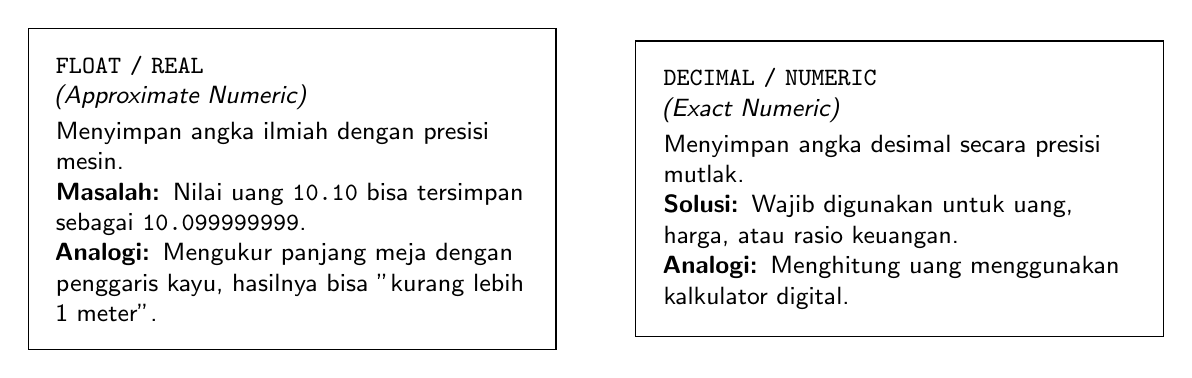
\begin{tikzpicture}[
			box/.style={rectangle, draw=black, text width=6cm, align=left, font=\sffamily\small, inner sep=10pt}
		]
		% FLOAT Box
		\node[box] (float) {
			\textbf{\texttt{FLOAT / REAL}} \\
			\textit{(Approximate Numeric)} \\[0.2em]
			Menyimpan angka ilmiah dengan presisi mesin. \\
			\textbf{Masalah:} Nilai uang \texttt{10.10} bisa tersimpan sebagai \texttt{10.099999999}. \\
			\textbf{Analogi:} Mengukur panjang meja dengan penggaris kayu, hasilnya bisa "kurang lebih 1 meter".
		};

		% DECIMAL Box
		\node[box, right=1cm of float] (decimal) {
			\textbf{\texttt{DECIMAL / NUMERIC}} \\
			\textit{(Exact Numeric)} \\[0.2em]
			Menyimpan angka desimal secara presisi mutlak. \\
			\textbf{Solusi:} Wajib digunakan untuk uang, harga, atau rasio keuangan. \\
			\textbf{Analogi:} Menghitung uang menggunakan kalkulator digital.
		};
	\end{tikzpicture}
	\caption{Perbandingan Filosofis antara FLOAT dan DECIMAL.}
\end{figure}

\section{Tipe Data String: Alokasi Memori yang Berbeda}

String (teks) adalah tipe data yang paling sering digunakan. Namun, SQL membedakan cara mengalokasikan memori untuk teks.

\subsection{\texttt{CHAR} vs \texttt{VARCHAR}: Memahami Lebar Memori}
\begin{itemize}
	\item \texttt{CHAR(n)}: Memori dipesan secara \textbf{tetap}. Jika kita memesan \texttt{CHAR(5)} dan menyimpan "dua", sistem akan menyimpannya sebagai "dua  " (ditambah 2 spasi).
	\item \texttt{VARCHAR(n)}: Memori dipesan secara \textbf{dinamis}. Jika kita memesan \texttt{VARCHAR(5)} dan menyimpan "dua", sistem hanya menggunakan 3 \textit{byte}.
\end{itemize}

\begin{figure}[H]
	\centering
	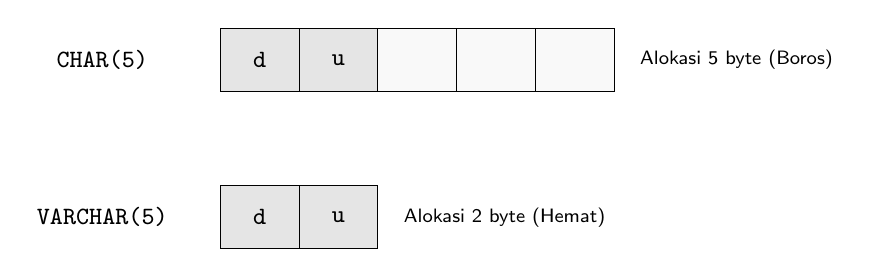
\begin{tikzpicture}[
			cell/.style={rectangle, draw=black, minimum width=1cm, minimum height=0.8cm, font=\ttfamily\small},
			label/.style={font=\sffamily\small\bfseries}
		]
		% CHAR (5)
		\node[label] at (-2, 2) {\texttt{CHAR(5)}};
		\node[cell, fill=gray!20] (c1) at (0,2) {d};
		\node[cell, fill=gray!20] (c2) at (1,2) {u};
		\node[cell, fill=gray!5] (c3) at (2,2) { };
		\node[cell, fill=gray!5] (c4) at (3,2) { };
		\node[cell, fill=gray!5] (c5) at (4,2) { };
		\node[font=\scriptsize\sffamily, right=0.2cm of c5] {Alokasi 5 byte (Boros)};

		% VARCHAR (5)
		\node[label] at (-2, 0) {\texttt{VARCHAR(5)}};
		\node[cell, fill=gray!20] (v1) at (0,0) {d};
		\node[cell, fill=gray!20] (v2) at (1,0) {u};
		\node[font=\scriptsize\sffamily, right=0.2cm of v2] {Alokasi 2 byte (Hemat)};
	\end{tikzpicture}
	\caption{Ilustrasi Alokasi Memori: "du" disimpan dalam \texttt{CHAR(5)} dan \texttt{VARCHAR(5)}.}
\end{figure}

\noindent\textbf{Aturan Emas:} Gunakan \texttt{CHAR} hanya untuk data yang panjangnya pasti (seperti Kode Negara 'ID', 'US', atau Kode Pos '29461'). Untuk Nama, Alamat, atau Email, gunakan \texttt{VARCHAR}.

\section{Tipe Data Waktu, Biner, dan Modern}

\subsection{Tanggal dan Waktu}
Jangan pernah menyimpan tanggal dalam bentuk string (teks). Selalu gunakan tipe data waktu agar operasi aritmatika tanggal (seperti mencari "selisih hari") bisa dilakukan.
\begin{itemize}
	\item \texttt{DATE}: Menyimpan tahun-bulan-tanggal (contoh: \texttt{2026-10-27}).
	\item \texttt{DATETIME / TIMESTAMP}: Menyimpan tanggal dan waktu lengkap hingga milidetik. Sangat penting untuk mencatat kapan sebuah transaksi terjadi.
\end{itemize}

\subsection{Tipe Data Khusus (Modern)}
Seiring berkembangnya aplikasi, SQL modern menambahkan tipe data khusus:
\begin{itemize}
	\item \texttt{JSON / JSONB} (PostgreSQL, MySQL): Untuk menyimpan data semi-terstruktur seperti konfigurasi aplikasi atau respons API.
	\item \texttt{UUID}: Untuk *Universally Unique Identifier*, sering digunakan sebagai ID yang tidak mudah ditebak (alternatif dari \texttt{AUTO\_INCREMENT}).
	\item \texttt{BLOB}: Untuk menyimpan file biner besar (gambar, dokumen PDF). \textit{Catatan: Menyimpan file di database seringkali kurang efisien dibanding menyimpan path file-nya saja.}
\end{itemize}

\section{Panduan Memilih Tipe Data (Decision Tree)}

Bagaimana cara cepat memilih tipe data yang tepat di dunia kerja? Ikuti alur pemikiran sederhana ini:

\begin{enumerate}
	\item \textbf{Apakah datanya berupa angka?}
	      \begin{itemize}
		      \item Jika untuk uang/harga: Gunakan \texttt{DECIMAL/NUMERIC}.
		      \item Jika untuk perhitungan ilmiah: Gunakan \texttt{FLOAT/DOUBLE}.
		      \item Jika hitungan biasa (usia, jumlah): Gunakan \texttt{INT}.
	      \end{itemize}
	\item \textbf{Apakah datanya berupa teks?}
	      \begin{itemize}
		      \item Jika panjangnya pasti (misal: Kode Provinsi 'KT'): Gunakan \texttt{CHAR(2)}.
		      \item Jika panjangnya bervariasi (Nama, Email): Gunakan \texttt{VARCHAR(255)}.
	      \end{itemize}
	\item \textbf{Apakah datanya berupa waktu?}
	      \begin{itemize}
		      \item Jika hanya tanggal lahir: Gunakan \texttt{DATE}.
		      \item Jika mencatat waktu transaksi: Gunakan \texttt{TIMESTAMP}.
	      \end{itemize}
	\item \textbf{Apakah datanya unik dan tidak berurutan?}
	      \begin{itemize}
		      \item Gunakan \texttt{UUID} agar tidak mudah diprediksi oleh peretas.
	      \end{itemize}
\end{enumerate}

\section{Kesimpulan}

Tipe data bukan sekadar urusan teknis saat menulis kueri \texttt{CREATE TABLE}. Ia adalah keputusan arsitektural yang menentukan seberapa cepat aplikasi berjalan, seberapa besar biaya penyimpanan yang dikeluarkan, dan seberapa aman data dari kesalahan pembulatan. Seorang \textit{software engineer} yang baik selalu memikirkan tipe data yang paling efisien, bukan hanya yang "bisa jalan".

\newpage
\section*{Referensi}
\addcontentsline{toc}{section}{Referensi}

\begin{thebibliography}{99}
	\bibitem{postgresql}
	The PostgreSQL Global Development Group. (2026). \textit{Chapter 8. Data Types}. PostgreSQL Documentation.

	\bibitem{oracle}
	Oracle Corporation. (2005). \textit{6 Datatypes}. Oracle Database SQL Quick Reference.

	\bibitem{microsoft}
	Microsoft. (2026). \textit{Working with Data Types}. Microsoft Learn.

	\bibitem{silberschatz}
	Silberschatz, A., Korth, H. F., \& Sudarshan, S. (2019). \textit{Database System Concepts} (7th ed.). McGraw-Hill Education.
\end{thebibliography}

\end{document}
